\documentclass[a4paper,12pt]{article}

\usepackage[russian]{babel}
\usepackage{cmap}
\usepackage[utf8]{inputenc}
\usepackage[usenames]{color}
\usepackage{tabularray}
\usepackage{xcolor}
\usepackage{graphicx} 
\usepackage{subfigure}
\usepackage{subcaption}

\usepackage[unicode]{hyperref} % цвета гиперссылок
\hypersetup{
	colorlinks,
	citecolor=black,
	filecolor=black,
	linkcolor=blue,
	urlcolor=black
}

\usepackage{geometry} % задаёт поля 
%\geometry{left=3cm}
%\geometry{right= 1.5cm}
%\geometry{top=2cm}
%\geometry{bottom=2cm} 

\usepackage{enumitem} % настраивает работу со списками:
\def\labelitemi{—} % ... задаёт длинное тире как стандартный маркер ненумерованного списка
\setlist{nolistsep} %  ... убирает дополнительный отступы между элементами списка


% удаляет названия и продолжение следует и т. для таблиц, будет только таблица без всего
\DefTblrTemplate{contfoot-text}{default}{}
\DefTblrTemplate{conthead-text}{default}{}
\DefTblrTemplate{caption}{default}{}
\DefTblrTemplate{conthead}{default}{}
\DefTblrTemplate{capcont}{default}{}


\title{Временные ряды потребления контента и усиление их прогнозирующих свойств построением сплит-моделей}
\author{В. Г. Мосин}
\date{}

%   \input{preamble.tex}
\begin{document}
	\maketitle
	\abstract{\noindent В На основании имеющегося временного ряда данных о потреблении контента на канале одного из ведущих хостингов построена регрессионная модель, аппроксимирующая его поведение кубическим полиномом. После разбиения данных на несколько непересекающихся классов построена серия подобных регрессионных моделей. Показано, что объединение частичных моделей приводит к существенному повышению точности аппроксимации.}
	
\tableofcontents
	
\section{Введение}
Временные ряды — это наборы данных, в которых значения измеряются в последовательные моменты времени. Они используются для анализа и прогнозирования переменных, которые изменяются во времени, таких как цены акций, количество продаж и другие. В анализе временных рядов применяются различные методы и модели для выявления скрытых закономерностей, трендов, цикличности, сезонности и шума в данных. Результаты таких исследований используются для предсказания будущих значений на основе предыдущих наблюдений.

\subsection{Теоретическая часть}

Если временной ряд обладает высокой волатильностью, то его анализ представляет определенные сложности из-за своих особенностей. Вот некоторые из них:
\medskip
\begin{enumerate}
	\item Шум и непостоянство. Высокая волатильность приводит к шуму и непостоянству в данных. Это затрудняет определение трендов и паттернов во временных рядах.
	\item Нестационарность. Временные ряды с высокой волатильностью часто бывают нестационарными, то есть их статистические свойства (среднее и дисперсия) меняются со временем. Нестационарность усложняет применение классических методов анализа, которые предполагают стационарность.
	\item Сложности прогнозирования. Волатильность создает большую неопределенность в прогнозировании будущих значений временных рядов. Это связано с тем, что даже небольшие изменения в данных или внешние факторы могут привести к значительным изменениям в прогнозах.
	\item Необходимость использования продвинутых методов. С учетом всех вышеперечисленных сложностей, анализ временных рядов с высокой волатильностью требует применения более продвинутых методов и моделей для достижения точных результатов.
\end{enumerate}
\medskip
Анализ временных рядов с высокой волатильностью может представлять определенные вызовы, но с правильным подходом можно извлечь полезную информацию. Один из таких подходов состоит в построении ансамбля моделей (см. [5], [6], [7]).
Ансамблирование моделей в машинном обучении — это метод, который объединяет предсказания нескольких моделей, чтобы получить более точный и стабильный прогноз. Он основан на идее, что объединение нескольких слабых моделей может привести к созданию более сильной и устойчивой модели. Процесс ансамблирования включает в себя два основных шага:
\medskip
\begin{enumerate}
	\item Создание множества моделей. Вместо использования единственной модели для предсказания, ансамбль создает несколько моделей, которые могут быть обучены с использованием различных методов или различных наборов данных. Например, можно использовать разные алгоритмы машинного обучения, разные фрагменты данных и т. д.
	\item Комбинирование предсказаний. После того как модели обучены, их предсказания объединяются для получения окончательного прогноза. 
\end{enumerate}
%\medskip
%Преимущества ансамблирования очевидны: они включают повышение точности предсказаний, устойчивость к шуму и выбросам, а так же, что самое важное,  улучшение обобщающей способности модели.  Заметим, что ансамблирование моделей является широко применяемым методом в машинном обучении и используется в различных задачах, включая классификацию, регрессию и анализ временных рядов (см. [3], [6], [7]).

\subsection{Постановки задачи}

\subsubsection{Предмет исследования} Мы исследуем данные о просмотрах образовательного контента на канале одного из ведущих хостингов. Данные представлены в виде временного ряда с дневной периодичностью с 2023-03-28 по 2023-06-28.
\subsubsection{Методика исследования} Для исследования мы применяем методы линейной и полиномиальной регрессии в два этапа. На первом этапе мы анализируем полные данные по всей выборке. На втором этапе мы разбиваем выборку на несколько фрагментов и анализируем их по отдельности, после чего агрегируем результаты.

\subsubsection{Цель исследования} Наша цель состоит в повышении прогнозирующей способности регрессионной модели временного ряда данных. Для этого мы сравниваем результаты моделирования, которые получаются на первом и втором этапах нашего исследования.

\subsection{Библиотеки}
Для выполнения вычислений и анализа данных мы пользуемся средой \texttt{Jupyter Notebook}, которая предоставляет удобные средства для работы с языком программирования Python и его главными библиотеками: \texttt{NumPy}, \texttt{Pandas}, \texttt{sklearn} и \texttt{matplotlib}. Благодаря этим инструментам, мы можем эффективно работать с данными, выполнять исследования и визуализировать результаты (см. [1], [2]).

%Библиотека \texttt{numpy} является одной из ключевых библиотек для научных вычислений и обработки массивов данных в языке программирования \texttt{Python}. Она предлагает эффективные структуры данных, алгоритмы и функции для операций с многомерными числовыми массивами.
%
%Библиотека \texttt{pandas}~--- одна из наиболее популярных и мощных библиотек для работы с данными в языке программирования \texttt{Python} (см. [1]). Она тесно взаимодействует с другими инструментами для вычислений и анализа данных на платформе \texttt{Python}, такими как \texttt{numpy}, \texttt{sklearn} и \texttt{matplotlib}. Это обеспечивает эффективную работу с информацией и применение различных алгоритмов и функций для анализа и визуализации данных.
%
%Библиотека \texttt{scikit-learn}, широко известная как \texttt{sklearn}, предоставляет обширный набор инструментов и функций для решения различных задач в языке программирования Python, таких как задачи классификации, регрессии, кластеризации и др. Мы используем эту библиотеку для решения регрессионных задач.

\section{Описание данных}
Данные содержат сведения о количестве просмотров образовательного контента на канале одного из ведущих хостингов, представленные в виде временного ряда. Период временного ряда — с 2023-03-28 по 2023-06-28, частота наблюдений~--- ежедневно.

\section{Алгоритм}
\subsection{Чтение данных}
Методом \texttt{read\_csv} библиотеки \texttt{pandas} загружаем в среду исполнения набор данных и формируем дата-фрейм. 

\noindent
%---------------------------------------
%---------------------------------------
\SetTblrInner{rowsep=3pt}
%---------------------------------------
\begin{longtblr}
	{
		colspec = {
			X[r,f]
			X[r,f,4] 
			X[r,f,4] 
			},
		width = 0.5\linewidth,
		rowhead = 1, 
		rowfoot = 0,
		row{odd} = {}, 
		row{even} = {},
		rows    = {font=\scriptsize},
		row{1}  = {font=\scriptsize\bfseries}
	}
	&
	Дата 
	& 
	Просмотры
	\\
	\hline[1pt]
	
	\textbf{0}   & 2023-03-28   & 1557
	\\
	\hline
	\textbf{1}   & 2023-03-29    & 1313   
	\\
	\hline
	\textbf{2}   & 2023-03-30    & 1248    
	\\
	\hline
	\textbf{...} & ...    & ...     & 
	\\
	\hline
	\textbf{91} & 2023-06-27    & 980    
	\\
	\hline
	\textbf{92} & 2023-06-28    & 902    
	\\
	\hline[1pt]
\end{longtblr}
%---------------------------------------
\noindent
Признак 'Дата' относится к строковому типу, признак 'Просмотры'~--- к типу целых чисел, пропущенных данных нет.



\subsection{Визуализация временного ряда}

Пользуясь методом \texttt{plot} библиотеки \texttt{matlpotlib}, визуализируем временной ряд: по горизонтали отложены номера дат, по вертикали~--- количество просмотров (см. рис. 1).

\begin{figure}[!h]
	\centering
	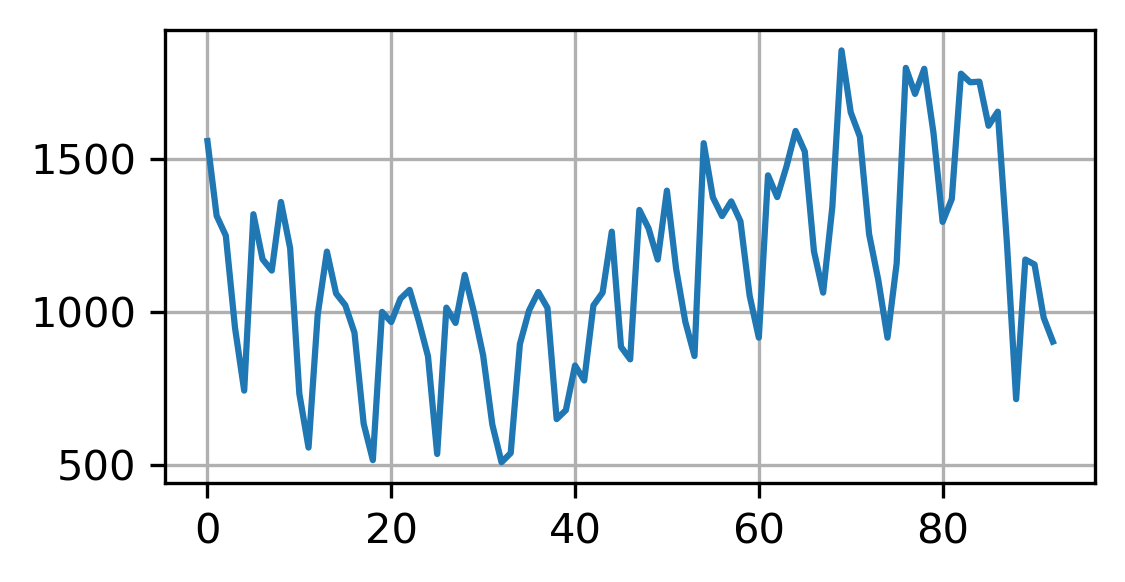
\includegraphics[width=0.7\linewidth]{pictures/Общая кривая}
		\caption{Временной ряд просмотров}
\end{figure}

\subsection{Построение и обучение моделей}
Мы проведем исследование и сравним несколько регрессионных моделей: сначала построим линейную модель, а затем две полиномиальные — квадратичную и кубическую.

\subsubsection{ Предварительная подготовка данных}
Данные признака 'Дата' являются строковыми, и мы не можем использовать этот признак в качестве независимой переменной регрессионной задачи, поскольку библиотека \texttt{sklearn} поддерживает только числовые данные. Мы добавляем в дата-фрейм столбец, совпадающий с индексом, и объявляем его признаком 'Номер':
\noindent
%---------------------------------------
%---------------------------------------
\SetTblrInner{rowsep=3pt}
%---------------------------------------
\begin{longtblr}
	{
		colspec = {
			X[r,f]
			X[r,f,4] 
			X[r,f,4]
			X[r,f,4]
		},
		width = 0.7\linewidth,
		rowhead = 1, 
		rowfoot = 0,
		row{odd} = {}, 
		row{even} = {},
		rows    = {font=\scriptsize},
		row{1}  = {font=\scriptsize\bfseries}
	}
	&
	Дата 
	& 
	Номер
	&
	Просмотры
	\\
	\hline[1pt]
	
	\textbf{0}   & 2023-03-28 & 1  & 1557
	\\
	\hline
	\textbf{1}   & 2023-03-29 &  2 & 1313   
	\\
	\hline
	\textbf{2}   & 2023-03-30 & 3  & 1248    
	\\
	\hline
	\textbf{...} & ...        & ... &  ...
	\\
	\hline
	\textbf{91} & 2023-06-27 & 92  & 980    
	\\
	\hline
	\textbf{92} & 2023-06-28 & 93  & 902    
	\\
	\hline[1pt]
\end{longtblr}
%---------------------------------------
\noindent
Визуально ничего не изменилось. Если посмотреть на рис. 1, то на нем и раньше по горизонтали откладывались не сами даты, а их номера. Зато теперь данные являются числовыми, и мы можем строить регрессионные модели.
\subsubsection{Линейная модель}
Сначала мы формируем одномерную регрессионную задачу с линейной моделью. Пользуясь методом \texttt{drop} библиотеки \texttt{pandas}, удаляем из дата-фрейма признаки 'Просмотры' и 'Дата', пользуясь методом \texttt{to\_numpy}, переводим оставшийся фрагмент в массив \texttt{numpy} и объявляем его левой частью регрессионной задачи (обозначение — \texttt{X}). В качестве правой части~--- наоборот,  используем признак 'Просмотры' (обозначение — \texttt{y}). Затем, пользуясь методом \texttt{LinearRegression} модуля \texttt{sklearn.linear\_model} из библиотеки \texttt{sklearn}, мы формируем объект \texttt{model} и, применяя к нему метод \texttt{fit}, обучаем модель на \texttt{X} и \texttt{y}. При помощи метода \texttt{score} мы вычисляем коэффициент детерминации: $R^2 = 0.22$, и наконец, средствами библиотеки \texttt{matplotlib} визуализируем модель (см. рис. 2(a)).

\subsubsection{Квадратичная  модель}
Полученный выше коэффициент детерминации кране низок. Чтобы усилить нашу модель, мы вводим еще один предиктор, равный квадрату предиктора  'Номер':

\noindent
%---------------------------------------
%---------------------------------------
\SetTblrInner{rowsep=3pt}
%---------------------------------------
\begin{longtblr}
	{
		colspec = {
			X[r,f]
			X[r,f,4] 
			X[r,f,4]
			X[r,f,4]
			X[r,f,4]
		},
		width = 0.85\linewidth,
		rowhead = 1, 
		rowfoot = 0,
		row{odd} = {}, 
		row{even} = {},
		rows    = {font=\scriptsize},
		row{1}  = {font=\scriptsize\bfseries}
	}
	&
	Дата 
	& 
	Номер
	&
	Квадрат номера
	&
	Просмотры
	\\
	\hline[1pt]
	
	\textbf{0}   & 2023-03-28 &  1 & 1    & 1557
	\\
	\hline
	\textbf{1}   & 2023-03-29 &  2 & 4    & 1313   
	\\
	\hline
	\textbf{2}   & 2023-03-30 &  3 & 9    & 1248    
	\\
	\hline
	\textbf{...} & ...        & ...&...   &...
	\\
	\hline
	\textbf{91} & 2023-06-27 & 92  & 8281 & 980    
	\\
	\hline
	\textbf{92} & 2023-06-28 & 93  & 8464 & 902    
	\\
	\hline[1pt]
\end{longtblr}
%---------------------------------------
\noindent
 Затем, повторяя действия, оцениваем (получается $R^2 = 0.25$, это лучше чем было, но по-прежнему очень мало) и визуализируем квадратичную модель (см. рис. 2(b)).

\subsubsection{Кубическая  модель}
Следующая попытка усилить модель состоит в том, что мы вводим еще один предиктор, равный кубу предиктора 'Номер':
\noindent
%---------------------------------------
%---------------------------------------
\SetTblrInner{rowsep=3pt}
%---------------------------------------
\begin{longtblr}
	{
		colspec = {
			X[r,f]
			X[r,f,4] 
			X[r,f,4]
			X[r,f,4]
			X[r,f,4]
			X[r,f,4]
		},
		width = 1\linewidth,
		rowhead = 1, 
		rowfoot = 0,
		row{odd} = {}, 
		row{even} = {},
		rows    = {font=\scriptsize},
		row{1}  = {font=\scriptsize\bfseries}
	}
	&
	Дата 
	& 
	Номер
	&
	Квадрат номера
	&
	Куб номера
	&
	Просмотры
	\\
	\hline[1pt]
	
	\textbf{0}   & 2023-03-28 &  1 & 1    & 1      & 1557
	\\
	\hline
	\textbf{1}   & 2023-03-29 &  2 & 4    & 8      & 1313   
	\\
	\hline
	\textbf{2}   & 2023-03-30 &  3 & 9    & 27     & 1248    
	\\
	\hline
	\textbf{...} & ...        & ...&...   &...     & ...
	\\
	\hline
	\textbf{91} & 2023-06-27 & 92  & 8281 & 753571 & 980    
	\\
	\hline
	\textbf{92} & 2023-06-28 & 93  & 8464 & 778688 & 902    
	\\
	\hline[1pt]
\end{longtblr}
%---------------------------------------
\noindent
После чего, повторяя действия, обучаем, оцениваем и визуализируем кубическую модель (см. рис. 2(c)).

На этот раз поучаем $R^2 = 0.48$. Это неудовлетворительно низкий результат. Причем, характер поведения кривой временного ряда таков, что кубическая парабола хорошо воспроизводит ее основной тренд, но не справляется с дневными колебаниями, и никакая алгебраическая кривая большей степени с ними тоже не справится, то есть, путь полиномиального усиления регрессионной модели следует признать тупиковым. 

\begin{figure}[!h]
	\centering
	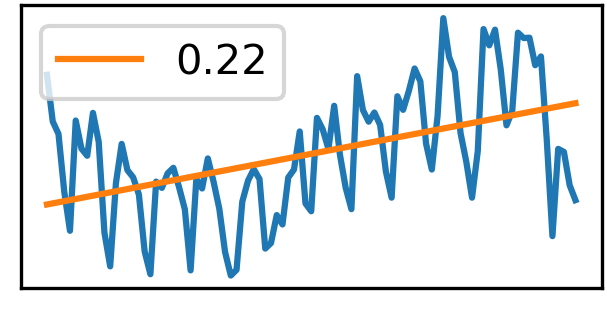
\includegraphics[width=0.25\linewidth]{pictures/1. Линейная модель}
	\hspace{0.01\linewidth}
	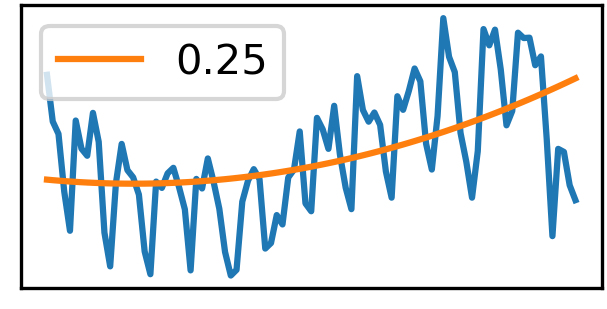
\includegraphics[width=0.25\linewidth]{pictures/2. Квадратичная модель}
	\hspace{0.01\linewidth}
	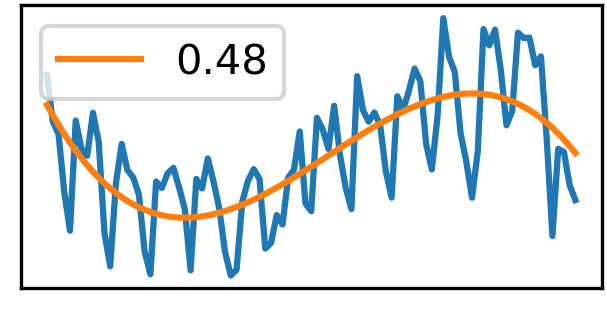
\includegraphics[width=0.25\linewidth]{pictures/3. Кубическая модель}
	\\
	\caption{Модели и их оценки}
\end{figure}
\noindent
Это значит, что нам нужны какие-то другие идеи для решения.

\subsection{Повторное чтение данных}
Мы прочитали данные из файла *.csv, а этот формат не содержит сведений о типе данных. Поэтому признак 'Дата' был прочитан как строковый, в тот момент как на самом деле он относится к типу дата-время. Чтобы изменить тип этого признака, мы методом \texttt{read\_csv} библиотеки \texttt{pandas} снова читаем данные из файла *.csv, но на этот раз используем атрибут \texttt{parse\_dates}, для того чтобы интерпретировать признак 'Дата' в нужном формате. Теперь признак 'Дата' имеет тип дата-время, а это значит, что он приобретает дополнительную информативность.

\subsection{Построение дополнительного признака}
Формат дата-время позволяет апеллировать к календарям и вычислять по любой дате день недели, который приходился (или еще придется) на эту дату. Для этого в библиотеке \texttt{pandas} есть метод \texttt{dt.dayofweek}, применяя который мы заносим в наш дата-фрейм еще один предиктор 'День недели':

\noindent
%---------------------------------------
%---------------------------------------
\SetTblrInner{rowsep=3pt}
%---------------------------------------
\begin{longtblr}
	{
		colspec = {
			X[r,f]
			X[r,f,4] 
			X[r,f,4]
			X[r,f,4]
		},
		width = 0.7\linewidth,
		rowhead = 1, 
		rowfoot = 0,
		row{odd} = {}, 
		row{even} = {},
		rows    = {font=\scriptsize},
		row{1}  = {font=\scriptsize\bfseries}
	}
	&
	Дата 
	& 
	День недели
	&
	Просмотры
	\\
	\hline[1pt]
	
	\textbf{0}   & 2023-03-28 & 1  & 1557
	\\
	\hline
	\textbf{1}   & 2023-03-29 &  2 & 1313   
	\\
	\hline
	\textbf{2}   & 2023-03-30 & 3  & 1248    
	\\
	\hline
	\textbf{...} & ...        & ... &  ...
	\\
	\hline
	\textbf{91} & 2023-06-27 & 1  & 980    
	\\
	\hline
	\textbf{92} & 2023-06-28 & 2  & 902    
	\\
	\hline[1pt]
\end{longtblr}
%---------------------------------------
\noindent
Дни недели закодированы, начиная с понедельника, таким образом: понедельник — 0, воскресенье — 6, и все промежуточные значения по порядку.


\subsection{Визуализация дополнительного признака}


На этом шаге мы применяем методы библиотеки \texttt{matplolib}, для того чтобы отметить чередование дней недели на общей кривой временного ряда (см. рис. 3).

\begin{figure}[!h]
	\centering
	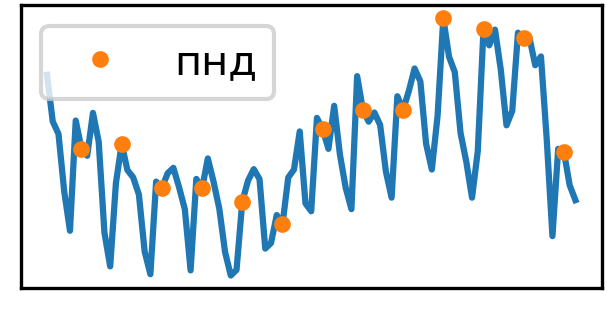
\includegraphics[width=0.25\linewidth]{pictures/0пнд}
	\hspace{0.01\linewidth}
	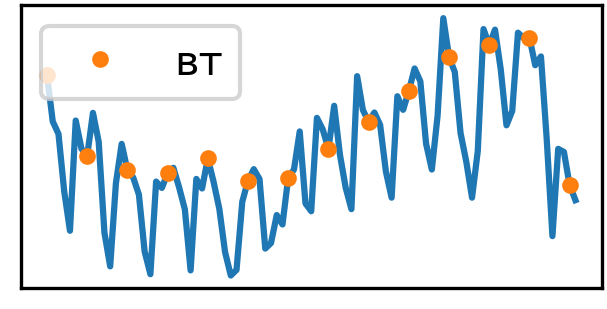
\includegraphics[width=0.25\linewidth]{pictures/1вт}
	\hspace{0.01\linewidth}
	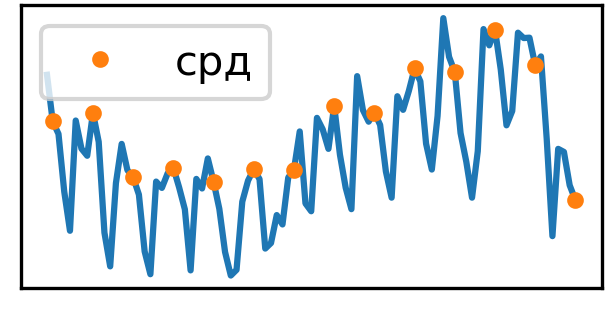
\includegraphics[width=0.25\linewidth]{pictures/2срд}
	\hspace{0.01\linewidth}
	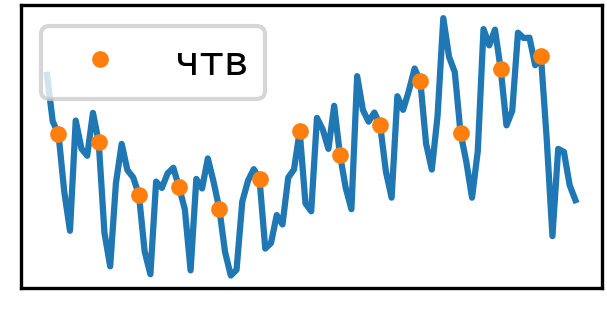
\includegraphics[width=0.25\linewidth]{pictures/3чтв}
	\hspace{0.01\linewidth}
	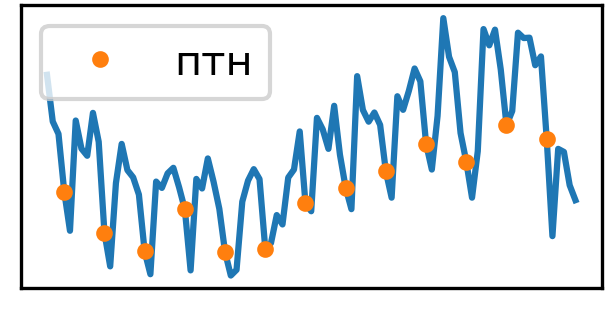
\includegraphics[width=0.25\linewidth]{pictures/4птн}
	\hspace{0.01\linewidth}
	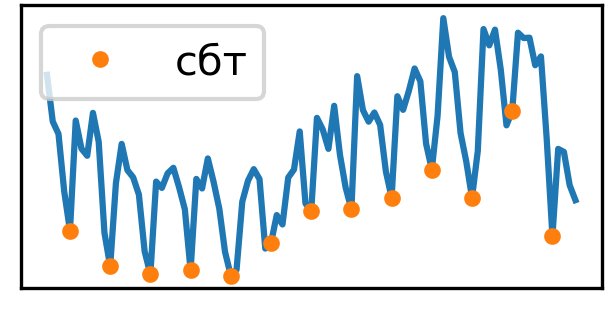
\includegraphics[width=0.25\linewidth]{pictures/5сбт}
	\hspace{0.01\linewidth}
	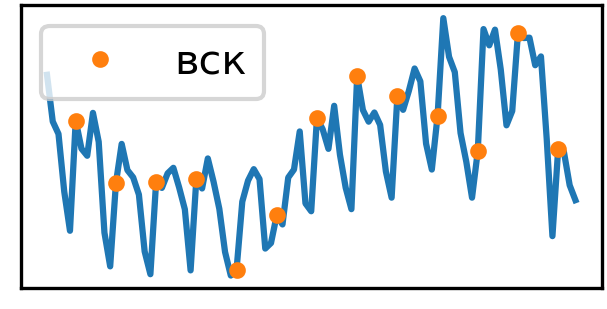
\includegraphics[width=0.25\linewidth]{pictures/6вск}
	\\
	\caption{Просмотры, локализованные по дням недели}
\end{figure}
\noindent
Бросается в глаза разительное отличие, например, суббот от вторников, хотя само по себе это наблюдение, конечно, не является неожиданным. Действительно, мы изучаем потребление образовательного контента, а образовательный процесс обладает естественной недельной цикличностью: по выходным студенты, как правило, отдыхают, а не учатся — отсюда глубокие пятничные и субботние провалы в потреблении. В начале недели студенты проявляют наибольшую активность, а воскресенье, хотя и выходной, но уже заставляет студентов задуматься о том, что завтра понедельник.

\subsection{Частичные модели}

Наша основная идея состоит в том, чтобы моделировать  потребление контента не на всем массиве данных, а на отдельных его фрагментах: построить и обучить отдельную модель для понедельников, отдельную — для вторников и так далее, по всем дням недели.

\subsubsection{Предварительная подготовка данных}

Здесь мы, так же как и выше применяем сквозную нумерацию объектов, добавляя в дата-фрейм дополнительный признак 'Номер'.

\noindent
%---------------------------------------
%---------------------------------------
\SetTblrInner{rowsep=3pt}
%---------------------------------------
\begin{longtblr}
	{
		colspec = {
			X[r,f]
			X[r,f,4] 
			X[r,f,4]
			X[r,f,4]
			X[r,f,4]
		},
		width = 0.85\linewidth,
		rowhead = 1, 
		rowfoot = 0,
		row{odd} = {}, 
		row{even} = {},
		rows    = {font=\scriptsize},
		row{1}  = {font=\scriptsize\bfseries}
	}
	&
	Дата 
	& 
	Номер
	&
	День недели
	&
	Просмотры
	\\
	\hline[1pt]
	
	\textbf{0}   & 2023-03-28 &  1 & 1    & 1557
	\\
	\hline
	\textbf{1}   & 2023-03-29 &  2 & 2    & 1313   
	\\
	\hline
	\textbf{2}   & 2023-03-30 &  3 & 3    & 1248    
	\\
	\hline
	\textbf{...} & ...        & ...&...   &...
	\\
	\hline
	\textbf{91} & 2023-06-27 & 92  & 1    & 980    
	\\
	\hline
	\textbf{92} & 2023-06-28 & 93  & 2    & 902    
	\\
	\hline[1pt]
\end{longtblr}
%---------------------------------------
\noindent

\subsubsection{Модель на понедельниках}
Прежде всего, пользуясь методом \texttt{loc} библиотеки \texttt{pandas}, мы выполняем локализацию дата-фрейма по условию 'День недели' = 0 и получаем локальный дата-фрейм: 

\noindent
%---------------------------------------
%---------------------------------------
\SetTblrInner{rowsep=3pt}
%---------------------------------------
\begin{longtblr}
	{
		colspec = {
			X[r,f]
			X[r,f,4] 
			X[r,f,4]
			X[r,f,4]
			X[r,f,4]
		},
		width = 0.85\linewidth,
		rowhead = 1, 
		rowfoot = 0,
		row{odd} = {}, 
		row{even} = {},
		rows    = {font=\scriptsize},
		row{1}  = {font=\scriptsize\bfseries}
	}
	&
	Дата 
	& 
	Номер
	&
	День недели
	&
	Просмотры
	\\
	\hline[1pt]
	
	\textbf{6}   & 2023-04-03 &	0	&6	&1171
	\\
	\hline
	\textbf{13}  & 2023-04-10  &	0	&13	&1196
	\\
	\hline
	\textbf{20}  & 2023-04-17  &	0	&20	&966
	\\
	\hline
	\textbf{...} & ...        & ...&...   &...
	\\
	\hline
	\textbf{83}  & 2023-06-19  & 0	& 83	&1749
	\\
	\hline
	\textbf{90}   & 2023-06-26	& 0	& 90	& 1154
	\\
	\hline[1pt]
\end{longtblr}
В нем, в отличие от полных данных не 93, а всего 13 записей, причем, номера  и даты следуют с шагом 7. Затем строим и обучаем кубическую модель, вычисляем ее метрику эффективности $R^2 = 0.79$ и визуализируем в виде кубической параболы (см. рис. 4(a)).


\subsubsection{Модели на остальных днях недели}

Повторяем в цикле по дням недели. Получаем еще 6 моделей (каждую на своей локализации), обучаем их, вычисляем метрики эффективности и визуализируем (см. рис. 4).


\begin{figure}[!h]
	\centering
	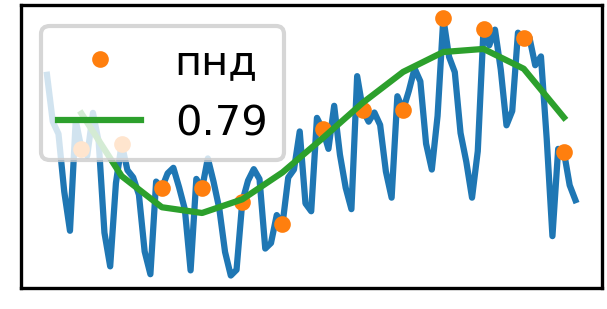
\includegraphics[width=0.25\linewidth]{pictures/0пндскор}
	\hspace{0.01\linewidth}
	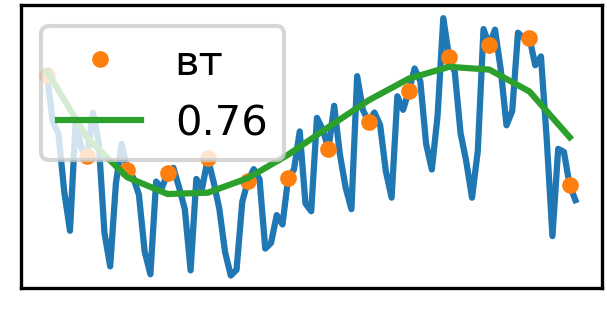
\includegraphics[width=0.25\linewidth]{pictures/1втскор}
	\hspace{0.01\linewidth}
	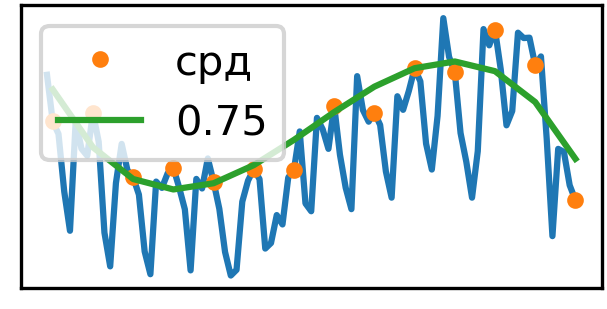
\includegraphics[width=0.25\linewidth]{pictures/2срдскор}
	\hspace{0.01\linewidth}
	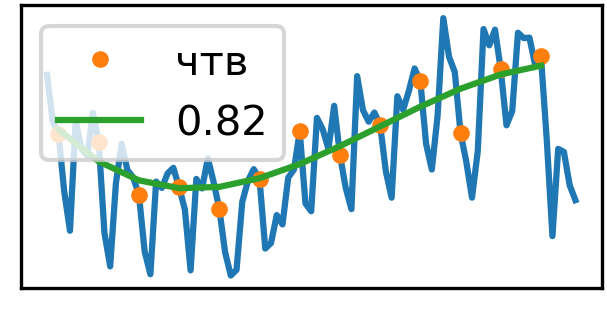
\includegraphics[width=0.25\linewidth]{pictures/3чтвскор}
	\hspace{0.01\linewidth}
	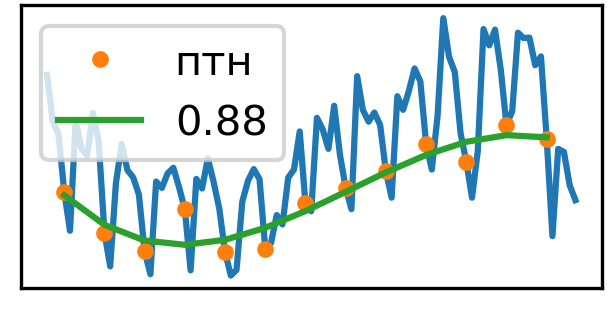
\includegraphics[width=0.25\linewidth]{pictures/4птнскор}
	\hspace{0.01\linewidth}
	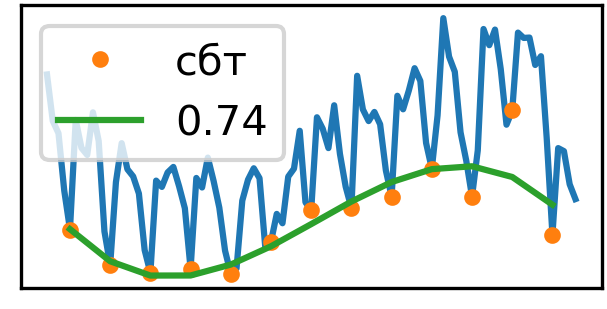
\includegraphics[width=0.25\linewidth]{pictures/5сбтскор}
	\hspace{0.01\linewidth}
	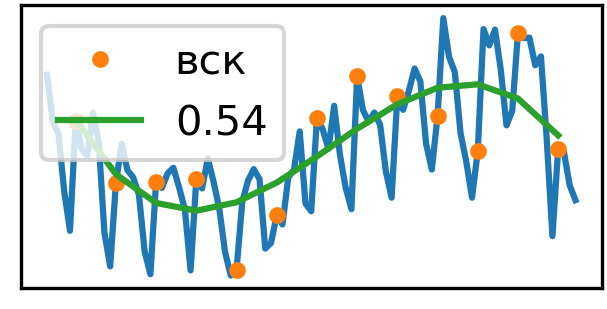
\includegraphics[width=0.25\linewidth]{pictures/6вскскор}
	\\
	\caption{Частичные модели и их оценки}
\end{figure}
\noindent

\section{Результаты}
Как линейная, так и полиномиальная модели потребления контента на полных данных оказались неудовлетворительными. Поэтому мы разбили данные на классы по дням недели, после чего построили и обучили частичные регрессионные модели третьей степени. Каждая из них по сравнению с начальной  полиномиальной  моделью обладает большим коэффициентом детерминации, однако, окончательная прогнозирующая способность всей совокупности частичных моделей оказывается еще выше (см. далее).

\subsection{Композиция моделей}
Итак, у нас есть семь моделей потребления контента в зависимости от дня недели. Пользуясь методом \texttt{coef\_} библиотеки \texttt{sklearn}, которая выводит наборы коэффициентов, а также методом \texttt{intercept\_}, который возвращает свободный член неоднородной регрессионной модели, мы можем описать потребление в виде явной функции от времени:

\noindent
%---------------------------------------
%---------------------------------------
\SetTblrInner{rowsep=3pt}
%---------------------------------------
\begin{longtblr}
	{
		colspec = {
			X[c,f, 2]
			X[l,f]
		},
		width = \linewidth,
		rowhead = 1, 
		rowfoot = 0,
		row{odd} = {}, 
		row{even} = {},
		rows    = {font=\scriptsize},
		row{1}  = {font=\scriptsize\bfseries}
	}
	Функция 
	& 
	Условие
	\\
	\hline[1pt]
	$1789.4219 - 85.5687 n + 2.2736 n^2 - 0.0153 n^3$
	& 
	если понедельник  
	\\
	\hline
	$1575.2983 - 61.1187 n + 1.7041 n^2 - 0.0118 n^3 $
	& 
	если вторник 
	\\
	\hline
    $1536.0606 - 57.3905 n + 1.6779 n^2 - 0.0119 n^3$
	& 
	если среда  
	\\
	\hline
	$1331.5792 - 32.1736 n + 0.8119 n^2 - 0.0046 n^3$
	& 
	если четверг 
	\\
	\hline
	$1018.4471 - 33.0131 n + 0.9056 n^2 - 0.0057 n^3$
	& 
	если пятница 
	\\
	\hline
	$0889.4622 - 41.2487 n + 1.2501 n^2 - 0.0089 n^3$
	& 
	если суббота 
		\\
	\hline
	$1621.7125 - 68.7657 n + 1.8182 n^2 - 0.0122 n^3$
	& 
	если воскресенье
	\\
	\hline[1pt]
\end{longtblr}
%---------------------------------------
\noindent
Здесь $n$ означает порядковый номер дня в ряду от 0 до 92. Эта функция не имеет аналитического описания, но это не делает ее менее привлекательной с точки зрения эффективности ее прогнозирующих свойств. Напротив, она эффективна именно потому, что не претендует на универсальность, а разнесена на семь записей в виде семи полиномов. 

\subsection{Метрика композиции моделей}

Чтобы получить общую метрику эффективности ансамбля моделей, нужно вспомнить определение коэффициента детерминации (см. [3], [4]):
$$
R^2 = 1 - S^*/ S’.
$$
Здесь $S^*$ — накопленный квадрат отклонения предсказанных значений от истинных значений целевой функции, а $S’$ — накопленный квадрат отклонения среднего значения целевой функции от ее истинных значений. Применяя метод \texttt{predict}  библиотеки \texttt{sklearn}, получаем предсказанные значения \texttt{y\_star} для каждой из частичных моделей, вычитаем их из истинных значений \texttt{y}, возводим в квадрат и суммируем методом \texttt{sum}. После этого в цикле по дням недели складываем все частичные суммы, получаем \texttt{S\_star} для всего ансамбля моделей. Для вычисления знаменателя \texttt{S\_line} применяем метод \texttt{mean}, который возвращает среднее значение массива, к правой части общей регрессионной задачи, отнимаем среднее значение от общего массива истинных значений, возводим результат в квадрат и суммируем элементы массива методом \texttt{sum}.

В результате имеем $R^2 = 0.82$. Если сравнить это значение с коэффициентом детерминации, полученным выше, на шаге, когда мы строили кубическую модель на полных данных (тогда получалось $R^2 = 0.48$), то окажется, что мы повысили метрику эффективности на 4 единицы в первом знаке после запятой! Это колоссальный рост коэффициента детерминации (обычно при повышении прогнозирующей способности регрессионной модели борьба ведется за хотя бы какой-нибудь сдвиг во втором знаке).

\section{Выводы}
Регрессионный анализ на частичных фрагментах данных с последующим построением ансамбля моделей обладает более высокой прогнозирующей способностью по сравнению с регрессионной моделью, построенной на полных данных по всей выборке. 
Это происходит, прежде всего, из-за учета локальной структуры данных: алгоритмы ансамблирования моделей, построенные на частичных фрагментах данных, точнее  учитывают локальную структуру данных и нелинейные зависимости в выборке. Модель, построенная на полных данных, может упустить некоторые особенности или несоответствия в данных, а это приводит к менее точным прогнозам.

\subsection{Обобщения}
В нашем исследовании нам удалось существенно повысить точность регрессионной модели после того, как мы включили в данные дополнительный такой показатель как день недели, что связано с недельным образовательным циклом. Однако ярко выраженная недельная цикличность наблюдается не только в образовании и потреблении образовательного контента, но и во многих других  общественных, экономических и производственных процессах. 
\medskip
\begin{enumerate}
	\item Например, в большинстве стран установлен 5-дневный рабочий график с выходными днями в субботу и воскресенье. Недельная цикличность имеет прямое отношение к этому графику.
	\item Потребление продуктов и услуг также имеет недельную цикличность: в выходные дни у потребителей больше времени для похода в рестораны, совершения покупок или посещения культурно-развлекательных мероприятий.
	\item Отдельного внимания заслуживает изучение транспортного потока: интенсивность транспортного движения существенно меняется в зависимости от дня недели. В будние дни транспортный поток обычно увеличивается, особенно в часы пик, в выходные дни и вечером движение обычно снижается.
	\item В туристической отрасли можно наблюдать выраженную недельную цикличность. Многие люди предпочитают ездить в путешествия на выходных, поэтому спрос на отели, рестораны и развлекательные мероприятия оказывается выше в эти дни.
\end{enumerate}
\medskip
И это лишь некоторые примеры процессов, в которых можно наблюдать ярко выраженную недельную цикличность.
 
\subsection{Рекомендации}

С учетом сказанного выше, вне зависимости от предметной области, если процесс обладает ярко выраженной недельной цикличностью, то целесообразно провести регрессионное моделирование, учитывая этот фактор. 

Прежде всего, абсолютно необходимо добавление фактора дня недели, так как включение этого фактора в регрессионную модель позволит учесть недельную цикличность. Для этого можно создать фиктивные переменные, соответствующие каждому дню недели, и включить их в модель в качестве предикторов. Это поможет учесть различия в поведении процесса по дням недели.

Кроме того, рекомендуется ансамблирование моделей, разделенных по дням недели. Это означает построение отдельных модели для каждого дня недели и использование их для прогнозирования в соответствующие дни. Когда такие модели построены и обучены, их можно объединить в виде ансамбля для получения общего прогноза.

Вместе с тем нужно отметить, что ансамблирование моделей может быть полезным, только если недельная цикличность действительно важна, и различия в поведении процесса действительно ярко выражены по дням недели. Следует помнить, что использование ансамблей моделей требует дополнительных ресурсов и анализа результатов, поэтому решение об организации ансамблирования нужно принимать на основе анализа данных, контекста и конкретных требований задачи прогнозирования.


\section{Литература}
\begin{enumerate}
	\item Хейдт М. Изучаем Pandas / М. Хейдт;  — Москва: ДМК Пресс, 2018. — 438 с.
	\item Бурков А. Машинное обучение без лишних слов / А. Бурков;  — СПб: Питер, 2020. — 192 с.
	\item Вьюгин, В. В. Математические основы теории машинного обучения и прогнозирования / В. В. Вьюгин; — М.: МЦИМО. — 2013. — 387 с. 
	\item Бринк Х. Машинное обучение / Х. Бринк, Дж. Ричардс, М. Феверолф  — СПб.: Питер, 2017. — 336 с.
	\item Газизов Д. И. Обзор методов статистического анализа временных рядов и проблемы, возникающие при анализе нестационарных временных рядов // Научный журнал. 2016. № 3 (4). С. 9--14.
	\item Фирулина М. М., Корунова Н. В. Разработка автоматизированных методов прогнозирования временных рядов // В сборнике: Прикладные информационные системы. Вторая Всероссийская НПК: сборник научных трудов. 2015. С. 401--405.
	\item Безверхий О. В., Курейчик В. М. Применение интеллектуальных информационных технологий при прогнозировании временных рядов // В сборнике: Искусственный интеллект в автоматизированных системах управления и обработки данных. Сборник статей Всероссийской научной конференции. В 2-х томах. Москва, 2022. С. 160--165.
\end{enumerate}




\end{document}